\documentclass[tikz,border=10pt]{standalone}
\usepackage{amsmath,amssymb}
\usepackage{tikz}
\usetikzlibrary{shapes.geometric,arrows.meta,positioning,calc}

\begin{document}
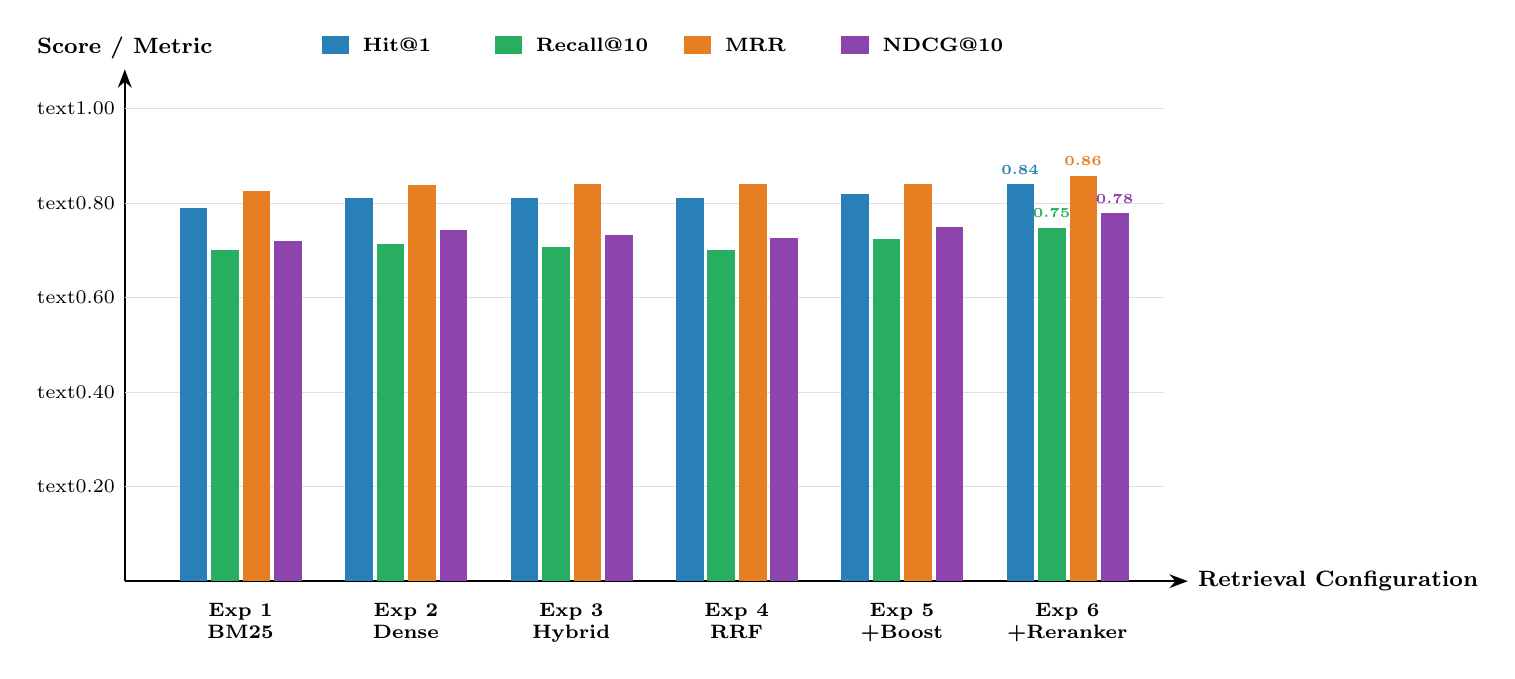
\begin{tikzpicture}[
    font=\sffamily\small,
    >=Stealth,
    bar/.style={rectangle, draw=none, rounded corners=2pt, minimum width=0.55cm},
    gridline/.style={draw=gray!25, thin}
]

% Coordinate system
% X: 6 configurations (BM25, Dense, Linear Hybrid, RRF, Entity Boost, Cross-Encoder)
% Y: 0.0 to 1.0 (scaled to 6cm)

\draw[thick, ->] (0,0) -- (13.5,0) node[right, font=\footnotesize\bfseries] {Retrieval Configuration};
\draw[thick, ->] (0,0) -- (0,6.5) node[above, font=\footnotesize\bfseries] {Score / Metric};

% Grid lines
\foreach \y/\val in {1.2/0.20, 2.4/0.40, 3.6/0.60, 4.8/0.80, 6.0/1.00} {
    \draw[gridline] (0,\y) -- (13.2,\y);
    \node[left, font=\scriptsize text=gray!80!black] at (0,\y) {\val};
}

% Configurations and their metric values (Canonical ground truth):
% Config 1: BM25 (x = 1.0)
% Hit@1: 0.79 -> 4.74
% Rec@10: 0.7003 -> 4.20
% MRR: 0.8271 -> 4.96
% NDCG@10: 0.7197 -> 4.32

% Colors
\definecolor{cHit}{RGB}{41, 128, 185}     % Blue
\definecolor{cRec}{RGB}{39, 174, 96}      % Green
\definecolor{cMRR}{RGB}{230, 126, 34}     % Orange
\definecolor{cNDCG}{RGB}{142, 68, 173}    % Purple

% Legend
\begin{scope}[shift={(2.5, 6.7)}]
    \fill[cHit] (0,0) rectangle (0.35,0.22);
    \node[right, font=\scriptsize\bfseries] at (0.4, 0.11) {Hit@1};
    \fill[cRec] (2.2,0) rectangle (2.55,0.22);
    \node[right, font=\scriptsize\bfseries] at (2.6, 0.11) {Recall@10};
    \fill[cMRR] (4.6,0) rectangle (4.95,0.22);
    \node[right, font=\scriptsize\bfseries] at (5.0, 0.11) {MRR};
    \fill[cNDCG] (6.6,0) rectangle (6.95,0.22);
    \node[right, font=\scriptsize\bfseries] at (7.0, 0.11) {NDCG@10};
\end{scope}

% Plot Bars function: xcenter, name, hit, rec, mrr, ndcg
% 1. BM25 (x = 1.3)
\fill[cHit]  (0.7,0) rectangle (1.05, 4.74);
\fill[cRec]  (1.1,0) rectangle (1.45, 4.20);
\fill[cMRR]  (1.5,0) rectangle (1.85, 4.96);
\fill[cNDCG] (1.9,0) rectangle (2.25, 4.32);
\node[below, font=\scriptsize\bfseries, align=center] at (1.47,-0.15) {Exp 1\\BM25};

% 2. Dense (x = 3.4)
\fill[cHit]  (2.8,0) rectangle (3.15, 4.86);
\fill[cRec]  (3.2,0) rectangle (3.55, 4.28);
\fill[cMRR]  (3.6,0) rectangle (3.95, 5.03);
\fill[cNDCG] (4.0,0) rectangle (4.35, 4.46);
\node[below, font=\scriptsize\bfseries, align=center] at (3.57,-0.15) {Exp 2\\Dense};

% 3. Linear Hybrid (x = 5.5)
\fill[cHit]  (4.9,0) rectangle (5.25, 4.86);
\fill[cRec]  (5.3,0) rectangle (5.65, 4.25);
\fill[cMRR]  (5.7,0) rectangle (6.05, 5.05);
\fill[cNDCG] (6.1,0) rectangle (6.45, 4.40);
\node[below, font=\scriptsize\bfseries, align=center] at (5.67,-0.15) {Exp 3\\Hybrid};

% 4. RRF (k=60) (x = 7.6)
\fill[cHit]  (7.0,0) rectangle (7.35, 4.86);
\fill[cRec]  (7.4,0) rectangle (7.75, 4.20);
\fill[cMRR]  (7.8,0) rectangle (8.15, 5.04);
\fill[cNDCG] (8.2,0) rectangle (8.55, 4.36);
\node[below, font=\scriptsize\bfseries, align=center] at (7.77,-0.15) {Exp 4\\RRF};

% 5. Entity Boost (x = 9.7)
\fill[cHit]  (9.1,0) rectangle (9.45, 4.92);
\fill[cRec]  (9.5,0) rectangle (9.85, 4.34);
\fill[cMRR]  (9.9,0) rectangle (10.25, 5.05);
\fill[cNDCG] (10.3,0) rectangle (10.65, 4.50);
\node[below, font=\scriptsize\bfseries, align=center] at (9.87,-0.15) {Exp 5\\+Boost};

% 6. Cross-Encoder (x = 11.8)
\fill[cHit]  (11.2,0) rectangle (11.55, 5.04);
\fill[cRec]  (11.6,0) rectangle (11.95, 4.49);
\fill[cMRR]  (12.0,0) rectangle (12.35, 5.15);
\fill[cNDCG] (12.4,0) rectangle (12.75, 4.67);
\node[below, font=\scriptsize\bfseries, align=center] at (11.97,-0.15) {Exp 6\\+Reranker};

% Annotations for Exp 6
\node[above, font=\tiny\bfseries, text=cHit] at (11.37, 5.04) {0.84};
\node[above, font=\tiny\bfseries, text=cRec] at (11.77, 4.49) {0.75};
\node[above, font=\tiny\bfseries, text=cMRR] at (12.17, 5.15) {0.86};
\node[above, font=\tiny\bfseries, text=cNDCG] at (12.57, 4.67) {0.78};

\end{tikzpicture}
\end{document}
